\section{Programmdokumentation und Funktionsbausteinbeschreibung}

\subsection{Hauptprogramm und eigene Funktionsbausteine}

Das Hauptprogramm stellt den Einstiegspunkt der Software dar. Aus diesem werden sämtliche Funktionen \bzw Funktionsbausteine aufgerufen, welche für das Verhalten der Anlage zuständig sind. Ausnahme ist lediglich das Programm mit den sicherheitsrelevanten Funktionen und Funktionsbausteinen.\\
\textbf{Wichtig ist anzumerken, dass in den Bildern gezeigtes Programm für eine Simulation eingesetzt wurde, und nicht mit einer realen Anlage genutzt werden darf. Dafür müssten sämtliche Variablen mit dem Suffix \textit{\glqq \_HMI\grqq{}} ersetzt werden durch die jeweilige Variable ohne den Suffix. Weitere Anpassungen für die Nutzung des Programms an einer realen Anlage wurden an den jeweiligen Funktionsbausteinen getätigt.}

\subsubsection{Main-File}

Das erste Netzwerk (\autoref{fig:Bild7.1}) setzt die Funktion des START-Drucktasters (S1) um. Über einen rücksetzdominanten FlipFlop wird die Betätigung des Tasters gespeichert, bis die Rücksetzbedingung (NOT S0) erfüllt ist. Ausgang des Netzwerkes ist eine Merkervariable (xM\_S1) mit der booleschen Information, dass \textbf{START} vom Nutzer gedrückt wurde.

\begin{figure}[H]
   \centering
   \fbox{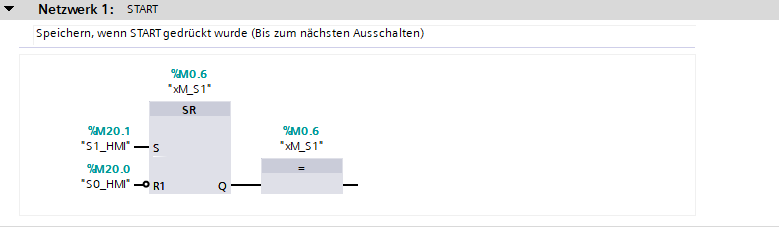
\includegraphics[width=0.8\textwidth]{Bilder/3. Programm/1. Hauptprogramm/main_1.png}}
   \caption[Starten der Anlage]{Starten der Anlage}
   \label{fig:Bild7.1}
\end{figure}

Im zweiten Netzwerk (\autoref{fig:Bild7.2}) wird der 5-Sekunden-Nachlauf des Förderbandes nach der Förderschnecke beim Ausschalten programmiert. Durch die Abfrage des Zustands des STOP-Leuchtdrucktasters (S0) wird das Schütz der Förderschnecke (K3) ausgeschaltet. Der STOP-Taster wurde als Öffner vorgesehen, folglich wird auf die negative Flanke getriggert. Sobald das Schütz (K3) ausgeschaltet ist, wird die Ausschaltverzögerung (TOF) gestartet. Nach Ablauf der 5-Sekunden wird das Schütz des Förderbandes (K4) ebenfalls ausgeschaltet.

\begin{figure}[H]
   \centering
   \fbox{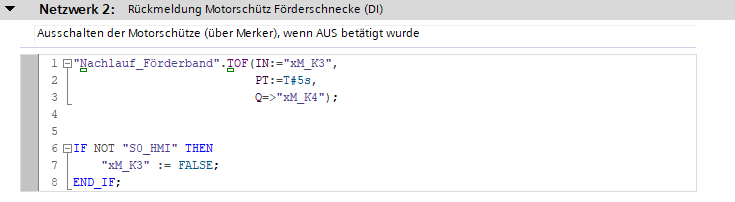
\includegraphics[width=0.8\textwidth]{Bilder/3. Programm/1. Hauptprogramm/main_2.png}}
   \caption[Stoppen der Anlage]{Stoppen der Anlage}
   \label{fig:Bild7.2}
\end{figure}

Im dritten Netzwerk (\autoref{fig:Bild7.3}) wurden Abfragen zu den Bedingungen für die Zustände der Anlage implementiert. Jede \textit{IF} \bzw \textit{ELSIF}-Bedingung fragt die Eintrittsvoraussetzungen eines Zustands ab. Diese können aus den Zustandsgraphen abgelesen werden. Sind die Bedingungen für einen Zustand erfüllt, wird der Funktionsbaustein \texttt{Zustände_DB()} mit einer Nummer aufgerufen. Die Nummer gibt an, um welchen Zustand es sich handelt. Folgende Zustände wurden Umgesetzt:

\begin{itemize}
    \item 0 - Betriebsbereiter Zustand
    \item 1 - Anlauf Förderband
    \item 2 - Anlauf Schnecke
    \item 3 - Schnecke Stop
    \item 4 - Förderband Stop
\end{itemize}

Der Nachlauf des Förderbandes wurde in keinem separaten Zustand umgesetzt, sondern ist in Netzwerk 2 (\autoref{fig:Bild7.2}) beim Stoppen der Anlage mit implementiert. \\
Der Anlauf der Schnecke erfolgt ebenfalls zeitverzögert (TON) und ist von Zeile 1 bis 3 im Netzwerk 3 (\autoref{fig:Bild7.3}) umgesetzt. Der Eingang der Einschaltverzögerung beinhaltet die gleichen Bedingungen wie der Zustand \textit{\glqq Anlauf Förderband\grqq{}}.

\begin{figure}[H]
   \centering
   \fbox{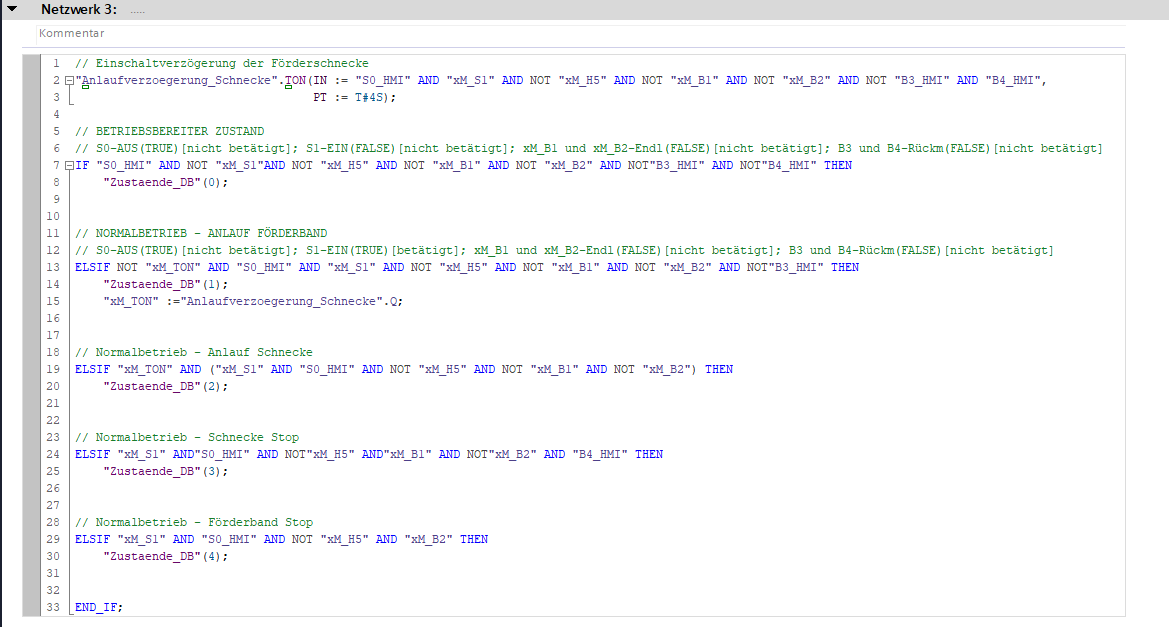
\includegraphics[width=0.95\textwidth]{Bilder/3. Programm/1. Hauptprogramm/main_3.png}}
   \caption[Abfrage der Zustandsbedingungen]{Abfrage der Zustandsbedingungen}
   \label{fig:Bild7.3}
\end{figure}

Das vierte Netzwerk (\autoref{fig:Bild7.4}) umfasst das Verhalten der Anlage im Fehlerfall. Dabei wird in drei Phasen unterschieden:
\begin{itemize}
    \item Fehler wird detektiert
    \item Fehler wird behoben
    \item Fehler wird quittiert
\end{itemize}

Im der ersten Phase blinkt der Leuchtmelder (H5) mit einer Frequenz von f = 1Hz. Dazu wird der Funktionsbaustein \texttt{Blinktakt()} aufgerufen. Sobald der Fehler behoben wurde, wird dies durch das dauerhafte Leuchten von H5 signalisiert. Gleichzeitig erfolgt das Blinken des QUITTIER-Leuchtdrucktasters (H2) mit selbiger Frequenz des Leuchtmelders H5 aus Phase 1. Sobald der QUITTIER-Leuchtdrucktaster (S2) gedrückt wurde, ist die Phase zwei beendet und die Anlage wird in Phase drei wieder in den betriebsbereiten Zustand versetzt.

\begin{figure}[H]
   \centering
   \fbox{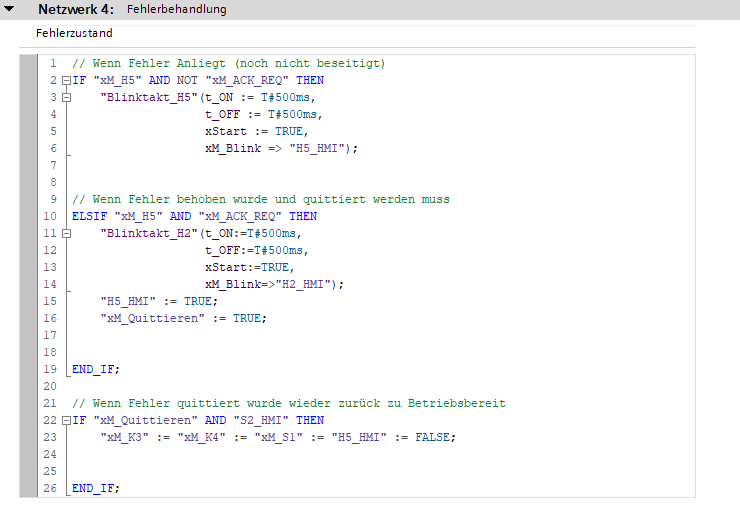
\includegraphics[width=0.8\textwidth]{Bilder/3. Programm/1. Hauptprogramm/main_4.png}}
   \caption[Beschreibung des Fehlerzustands]{Beschreibung des Fehlerzustands}
   \label{fig:Bild7.4}
\end{figure}

Das Netzwerk Fünf (\autoref{fig:Bild7.5}) ist lediglich im simulierten Anlagenzustand anzuwenden und ermöglicht die Rückmeldung der geschalteten Schütze (K3 und K4) durch die Variablen (B3 und B4). Im realen Anlagenbetrieb werden die Rückmeldungen automatisch durchgeführt, folglich ist dieses Netzwerk zu entfernen.

\begin{figure}[H]
   \centering
   \fbox{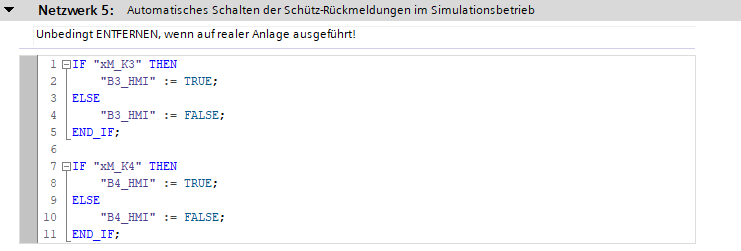
\includegraphics[width=0.8\textwidth]{Bilder/3. Programm/1. Hauptprogramm/main_5.png}}
   \caption[Setzen der Rückmeldungen der Schütze]{Setzen der Rückmeldungen der Schütze}
   \label{fig:Bild7.5}
\end{figure}

\subsubsection{Funktionsbaustein der Zustände}

Der Funktionsbaustein \texttt{Zustände_DB()} (\autoref{fig:Bild7.6}) umfasst die Implementierung der Zustände gemäß der Zustandsgraphen. Im Main-File werden entsprechend Integer-Werte von Null bis Vier vergeben. Anhand dieser Werte wird durch eine CASE-Anweisung der richtige Zustand ermittelt und die jeweiligen notwendigen Variablen auf TRUE oder FALSE gesetzt. Sofern die Anlage keinen dieser Zustände zugeordnet werden kann, wird über die ELSE-Abfrage eine Textnachricht im Terminal der SPS zurückgegeben. Die Anlage wird durch die Safety-Baugruppen ausgeschaltet und in einen sicheren Zustand versetzt.

\begin{figure}[H]
   \centering
   \fbox{\includegraphics[width=0.7\textwidth]{Bilder/3. Programm/1. Hauptprogramm/Zustände.png}}
   \caption[Funktionsbaustein Zustände\_DB()]{Funktionsbaustein Zustände\_DB()}
   \label{fig:Bild7.6}
\end{figure}

\subsubsection{Blinker-Funktionsbaustein}

Zuletzt wurde ein Funktionsbaustein für eine Blinker-Funktionalität umgesetzt (\autoref{fig:Bild7.7}). Über diesen ist es möglich per Aufruf von \texttt{Blinktakt()} ein Blinksignal zu generieren. Dem Funktionsbaustein kann eine Ein-Zeit (t\_ON) und eine Aus-Zeit (t\_OFF) mitgegeben werden, um den Blinktakt zu setzen. Über \textit{xStart} wird der Blinker aktiviert. Die Ausgangsvariable (xM\_Blink) liefert das generierte Blinksignal. \\
Eingesetzt wird der Funktionsbaustein für den \textbf{START-Leuchtdrucktaster}, den \textbf{Fehlerleuchtmelder} und den \textbf{QUITTIER-Leuchtdrucktaster}.

\begin{figure}[H]
   \centering
   \fbox{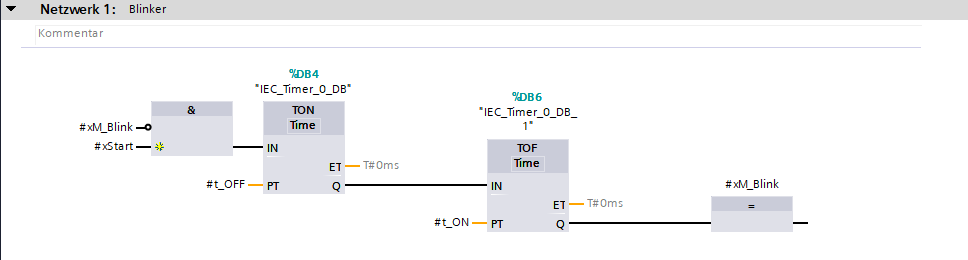
\includegraphics[width=0.8\textwidth]{Bilder/3. Programm/1. Hauptprogramm/Blinker.png}}
   \caption[Funktionsbaustein Blinker()]{Funktionsbaustein Blinker()}
   \label{fig:Bild7.7}
\end{figure}

\clearpage

\subsection{Safety-Programm}

\subsubsection{Grundlagen sichere Programme}

Das Sicherheitsprogramm wird parallel zum Hauptprogramm auf einer sogenannten F-CPU (fehlersichere CPU) ausgeführt. Es besitzt meist eine kürzere Zykluszeit und kann über Interrupts in das Hauptprogramm eingreifen, falls dies erforderlich ist (siehe \autoref{fig:Bild7.8}).

\begin{figure}[H]
   \centering
   \fbox{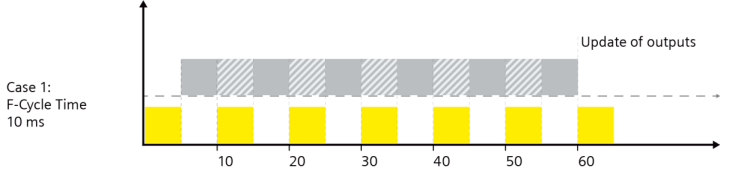
\includegraphics[width=0.8\textwidth]{Bilder/3. Programm/2. Safety/Zykluszeit_Safety.png}}
   \caption[Zykluszeit Sicherheitsprogramm]{Einfluss der Zykluszeit des Sicherheitsprogramms auf das Standard- Anwenderprogramm}
   \label{fig:Bild7.8}
\end{figure}

\subsubsection{Struktur von Sicherheitsprogrammen}

Ein Sicherheitsprogramm besteht zur Strukturierung aus einer oder zwei F‑Ablaufgruppen. 

Jede F‑Ablaufgruppe enthält:

\begin{itemize}
    \item F‑Bausteine, die von Ihnen mit FUP oder KOP erstellt werden oder aus der Projektbibliothek oder globalen Bibliotheken eingefügt werden
    \item F‑Bausteine, die automatisch ergänzt werden (F‑Systembausteine F‑SBs, automatisch generierte F‑Bausteine, F‑Ablaufgruppeninfo-DB und F‑Peripherie‑DBs)
\end{itemize}

\begin{figure}[H]
   \centering
   \fbox{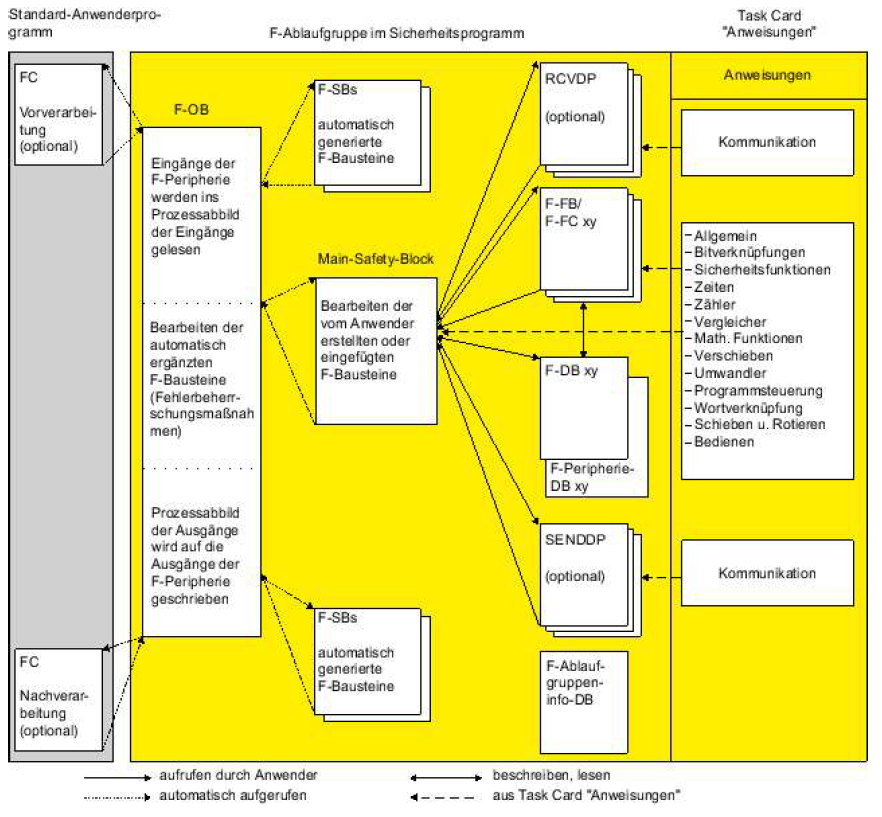
\includegraphics[width=0.95\textwidth]{Bilder/3. Programm/2. Safety/F-Ablaufgruppe.png}}
   \caption[Aufbau Sicherheitsprogramm]{Schematischen Aufbau eines Sicherheitsprogramms \bzw einer F‑Ablaufgruppe für eine F-CPU S7-1200/1500}
   \label{fig:Bild7.9}
\end{figure}

\clearpage

\subsubsection{Datenaustausch: Anwenderprogramm - Sicherheitsprogramm}

Es besteht die Möglichkeit, Daten zwischen dem Sicherheits- und Standard- Anwenderprogramm auszutauschen. Dazu können Variablen aus DBs, F-DBs sowie Merker verwendet werden:

\renewcommand{\arraystretch}{1.3}
\begin{table}[H]
    \centering
    \scalebox{0.8}{%
    \begin{tabular}{|l|cc|cc|}
        \hline
        & \multicolumn{2}{c|}{\textbf{Vom Standard-Anwenderprogramm aus}}
        & \multicolumn{2}{c|}{\textbf{Vom Sicherheitsprogramm aus}} \\
        \hline
        & \multicolumn{1}{c|}{\textbf{lesend}}
        & \textbf{schreibend}
        & \multicolumn{1}{c|}{\textbf{lesend}}
        & \textbf{schreibend}
        \\
        \hline
        Variable aus DB
        & \multicolumn{1}{c|}{zulässig}
        & zulässig
        & \multicolumn{2}{l|}{\makecell[l]{entweder lesend \underline{oder} schreibend auf eine \\ Variable aus dem DB}}
        \\
        \hline
        Variable aus F-DB
        & \multicolumn{1}{c|}{zulässig}
        & \textbf{nicht zulässig}
        & \multicolumn{1}{c|}{zulässig}
        & zulässig
        \\
        \hline
        Merker
        & \multicolumn{1}{c|}{zulässig}
        & zulässig
        & \multicolumn{2}{l|}{\makecell[l]{entweder lesend \underline{oder} schreibend auf einen \\ Merker}}
        \\
        \hline
    \end{tabular}%
    }
    \caption[Datenaustausch zwischen Sicherheits- und Standard-Anwenderprogramm]{Datenaustausch zwischen Sicherheits- und Standard-Anwenderprogramm}
    \label{tab:7.1}
    \
\end{table}
\renewcommand{\arraystretch}{1}

Außerdem besteht die Möglichkeit, auf das Prozessabbild der Standard- und F-Peripherie zuzugreifen:

\renewcommand{\arraystretch}{1.3}
\begin{table}[H]
    \centering
    \scalebox{0.8}{%
    \begin{tabular}{|l|c|cc|cc|}
        \hline
        &
        & \multicolumn{2}{c|}{\textbf{Vom    Standard-Anwenderprogramm aus}}
        & \multicolumn{2}{c|}{\textbf{Vom Sicherheitsprogramm aus}}
        \\ \hline
        &
        & \multicolumn{1}{c|}{\textbf{lesend}}
        & \textbf{schreibend}
        & \multicolumn{1}{c|}{\textbf{lesend} }
        & \textbf{schreibend}
        \\ \hline
        \multirow{2}{*}{\makecell[l]{Prozessabbild\\Standardperipherie}}
        & PAE
        & \multicolumn{1}{c|}{zulässig}
        & zulässig
        & \multicolumn{1}{c|}{zulässig}
        & \textbf{nicht zulässig}
        \\ \cline{2-6} 
        & PAA
        & \multicolumn{1}{c|}{zulässig}
        & zulässig 
        & \multicolumn{1}{c|}{\textbf{nicht zulässig}}
        & zulässig            
        \\ \hline
        \multirow{2}{*}{\makecell[l]{Prozessabbild\\F-Peripherie}}
        & PAE
        & \multicolumn{1}{c|}{zulässig}
        & \textbf{nicht zulässig}
        & \multicolumn{1}{c|}{zulässig}
        & \textbf{nicht zulässig}
        \\ \cline{2-6} 
        & PAA
        & \multicolumn{1}{c|}{zulässig}   
        & \textbf{nicht zulässig} 
        & \multicolumn{1}{c|}{\textbf{nicht zulässig}} 
        & zulässig           
        \\ \hline
        \end{tabular}%
    }
    \caption[Zugriff auf Prozessabbild der Standardperipherie und F-Peripherie]{Zugriff auf Prozessabbild der Standardperipherie und F-Peripherie}
    \label{tab:7.2}
\end{table}
\renewcommand{\arraystretch}{1}

Zur Entkopplung des Anwender- vom Sicherheitsprogramm wird empfohlen, für den Datenaustausch Übergabe-Datenbausteine zu definieren.

\clearpage

\subsubsection{Variablen der F-Peripherie-DBs}
\renewcommand{\arraystretch}{1.3}
\begin{table}[H]
    \centering  
    \scalebox{0.8}{%
    \begin{tabular}{|l|l|l|l|c|}
        \hline
        \multicolumn{1}{|c|}{}
        & \multicolumn{1}{c|}{\textbf{Variable}}
        & \multicolumn{1}{c|}{\textbf{Datentyp}}
        & \multicolumn{1}{c|}{\textbf{Funktion}}
        & \textbf{Startwert}
        \\ \hline
        \multirow{5}{*}{\begin{tabular}[c]{@{}l@{}}Variablen, die\\ Sie beschrei-\\ ben kön-\\ nen/müssen\end{tabular}}
        & PASS\_ON
        & BOOL
        & 1 = Passivierung aktivieren
        & 0 
        \\ \cline{2-5} 
        & ACK\_NEC
        & BOOL
        & \begin{tabular}[c]{@{}l@{}}1 = Quittierung für Wiedereingliederung\\ erforderlich bei F-Peripherie-/Kanalfehlern\end{tabular}
        & 1
        \\ \cline{2-5} 
        & ACK\_REI
        & BOOL
        & 1 = Quittierung für Wiedereingliederung
        & 0 
        \\ \cline{2-5} 
        & IPAR\_EN
        & BOOL
        & \begin{tabular}[c]{@{}l@{}}Variable für Umparametrierung fehlersiche-\\ rer DP-Normslaves/IO-Normdevices bzw.\\ bei SM 336; F-AI 6x0/4 ... 20 mA HART\\ zur Freigabe der HART-Kommunikation\end{tabular}
        & 0 
        \\ \cline{2-5} 
        & DISABLE*
        & BOOL
        & 1 = F-Peripherie deaktivieren
        & 0 
        \\ \hline
        \multirow{8}{*}{\begin{tabular}[c]{@{}l@{}}Variablen, die\\ Sie auswerten\\ können\end{tabular}}
        & PASS\_OUT
        & BOOL
        & Passivierungsausgang
        & 1 
        \\ \cline{2-5} 
        & QBAD
        & BOOL 
        & 1 = Ersatzwerte werden ausgegeben
        & 1 
        \\ \cline{2-5}
        & ACK\_REQ
        & BOOL
        & \begin{tabular}[c]{@{}l@{}}1 = Quittierungsanforderung für Wiederein-\\ gliederung\end{tabular} & 0 \\ \cline{2-5} 
        & IPAR\_OK
        & BOOL
        & \begin{tabular}[c]{@{}l@{}}Variable für Umparametrierung fehlersiche-\\ rer DP-Normslaves/IO-Normdevices bzw.\\ bei SM 336; F-AI 6x0/4 ... 20 mA HART\\ zur Freigabe der HART-Kommunikation\end{tabular}
        & 0 
        \\ \cline{2-5}
        & DIAG
        & BYTE
        & Nicht fehlersichere Serviceinformation
        & 0
        \\ \cline{2-5}
        & DISABLED*
        & BOOL
        & 1 = F-Peripherie ist deaktiviert
        & 0 
        \\ \cline{2-5}
        & QBAD\_I\_xx
        & BOOL
        & \begin{tabular}[c]{@{}l@{}}1 = Ersatzwerte werden ausgegeben auf\\ Eingangskanal xx (S7-300/400)\end{tabular}
        & 1 
        \\ \cline{2-5}
        & QBAD\_O\_xx
        & BOOL
        & \begin{tabular}[c]{@{}l@{}}1 = Ersatzwerte werden ausgegeben auf\\ Ausgangskanal xx (S7-300/400)\end{tabular}
        & 1
        \\ \hline
        \multicolumn{3}{l}{* ab Safety-System-Version V2.1 für S7-1200/1500}
    \end{tabular}%
   
    }
    \caption[Variablen der F-Peripherie-DBs]{Variablen der F-Peripherie-DBs}
    \label{tab:7.3}
\end{table}
\renewcommand{\arraystretch}{1}

\textbf{PASS\_ON:}\\
Mit der Variable PASS\_ON können Sie eine Passivierung einer F-Peripherie, z. B. abhängig von bestimmten Zuständen in Ihrem Sicherheitsprogramm, aktivieren.\\
Sie können über die Variable PASS\_ON im F-Peripherie-DB nur die gesamte F-Peripherie passivieren, kanalgranulare Passivierung ist nicht möglich.\\
Solange PASS\_ON = 1 ist, erfolgt eine \textbf{Passivierung} der zugehörigen F-Peripherie.\\

\textbf{ACK\_NEC:}\\
Wenn von der F-Peripherie ein F-Peripheriefehler erkannt wird, erfolgt eine \textbf{Passivierung} der betroffenen F-Peripherie. Wenn Kanalfehler erkannt werden, erfolgt bei projektierter kanalgranularer Passivierung eine Passivierung der betroffenen Kanäle, bei Passivierung der gesamten F-Peripherie eine Passivierung aller Kanäle der betroffenen F-Peripherie. Nach Behebung des F-Peripherie- /Kanalfehlers erfolgt die \textbf{Wiedereingliederung} der betroffenen F-Peripherie abhängig von ACK\_NEC:
\begin{itemize}
    \item Mit ACK\_NEC = 0 können Sie eine \textbf{automatische Wiedereingliederung} parametrieren.
    \item Mit ACK\_NEC = 1 können Sie eine \textbf{Wiedereingliederung} durch eine \textbf{Anwenderquittierung} parametrieren.
\end{itemize}

\textbf{ACK\_REI}:\\
Wenn vom F-System für eine F-Peripherie ein Kommunikationsfehler oder ein F-Peripheriefehler erkannt wird, erfolgt eine Passivierung der betroffenen F-Peripherie. Wenn Kanalfehler erkannt werden, erfolgt bei projektierter kanalgranularer Passivierung eine Passivierung der betroffenen Kanäle, bei Passivierung der gesamten F-Peripherie eine Passivierung aller Kanäle der betroffenen F-Peripherie. Für eine \textbf{Wiedereingliederung} der F-Peripherie/Kanäle der F-Peripherie nach Behebung der Fehler ist eine \textbf{Anwenderquittierung} mit positiver Flanke an der Variablen ACK\_REI des F-Peripherie-DBs erforderlich:
\begin{itemize}
    \item nach Kommunikationsfehlern immer
    \item nach F-Peripherie-/Kanalfehlern nur bei Parametrierung "Kanalfehler Quittierung = Manuell"\:bzw. ACK\_NEC = 1
\end{itemize}
Bei einer Wiedereingliederung nach Kanalfehlern werden alle Kanäle, deren Fehler beseitigt wurden, wiedereingegliedert.\\
Eine Quittierung ist erst möglich, wenn die Variable ACK\_REQ = 1 ist.\\

\textbf{IPAR_EN:}\\
Die Variable IPAR\_EN entspricht der Variablen iPAR\_EN\_C im Busprofil PROFIsafe, ab PROFIsafe Specification V1.20.\\

\textbf{Fehlersichere DP-Normslaves/IO-Normdevices}\\
Wann Sie diese Variable bei einer Umparametrierung von fehlersicheren DP-Normslaves/IO-Normdevices setzen/rücksetzen müssen, entnehmen Sie der PROFIsafe Specification ab V1.20 bzw. der Dokumentation zum fehlersicheren DP-Normslave/IO-Normdevice.\\
Beachten Sie, dass durch IPAR\_EN = 1 keine Passivierung der betroffenen F-Peripherie ausgelöst wird.\\
Soll bei IPAR\_EN = 1 passiviert werden, müssen Sie die Variable PASS\_ON = 1 setzen.\\

\textbf{DISABLE:}\\
Mit der Variable DISABLE können Sie eine F-Peripherie deaktivieren.\\
Solange DISABLE = 1 ist, erfolgt eine \textbf{Passivierung} der zugehörigen F-Peripherie.\\
In den Diagnosepuffer der F-CPU werden zu dieser F-Peripherie keine Diagnoseeinträge des Sicherheitsprogramms (z. B. wegen Kommunikationsfehler) mehr eingetragen.\\
Bereits vorhandene Diagnoseeinträge werden als gehend gekennzeichnet.\\

\textbf{QBAD:}\\
Bei einer Passivierung geht die F-Peripherie in den fehlersicheren Zustand. Nach Fehlerbehebung kann diese wieder eingegliedert werden.\\
Für die Wiedereingliederung existieren verschiedene Möglichkeiten. Dabei ist zu berücksichtigen, ob die F-Peripherie das PROFIsafe-Profil RIOforFA-Safety unterstützt.\\
Die Dezentrale Peripherie ET 200SP, hier: F-DI8x24 V DC verfügt über KEIN RIOforFA-Safety Profil.\\
Kommt es an einer F-Peripherie zu einem Fehler (z. B. zu einem Kanalfehler) geht die F-Peripherie (bzw. der betroffene Kanal) in den sicheren Zustand. In diesem Zustand der „Passivierung“ werden statt der Prozesswerte automatisch Ersatzwerte ausgegeben.\\
Nach Beseitigung des Fehlers, der zur Passivierung führte, kann die Umschaltung von Ersatzwerte auf Prozesswerte erfolgen. Die Umschaltung kann automatisch oder nach einer Anwenderquittierung im Sicherheitsprogramm erfolgen.\\
Begriffe für die Umschaltung sind „Wiedereingliederung“ oder auch „Reintegration“.

\renewcommand{\arraystretch}{1.3}
\begin{table}[H]
    \centering
    \scalebox{0.9}{%
    \begin{tabular}{|l|l|}
        \hline
        \multicolumn{1}{|c|}{\textbf{Ersatzwertausgabe nach:}}
        & \multicolumn{1}{c|}{\textbf{\begin{tabular}[c]{@{}c@{}}F-Peripherie ohne Profil\\ "RIOforFA-Safety" mit FCPUs\\ S7-1200/1500\end{tabular}}} \\ \hline
        Anlauf des F-Systems
        & \multirow{4}{*}{\begin{tabular}[c]{@{}l@{}}QBAD und PASS\_OUT = 1,\\ DISABLED \textbf{unverändert},\\ für \textbf{alle} Kanäle gilt:\\ - Kanalwert = Ersatzwert (0)\\ - Wertstatus = 0*\end{tabular}}
        \\ \cline{1-1}
        Kommunikationsfehlern
        & \\ \cline{1-1}
        F-Peripheriefehlern
        & \\ \cline{1-1}
        \begin{tabular}[c]{@{}l@{}}Kanalfehlern bei Projektierung\\ Passivierung der gesamten F-Peripherie\end{tabular}
        & \\ \hline
        \begin{tabular}[c]{@{}l@{}}Kanalfehlern bei Projektierung\\ kanalgranulare Passivierung\end{tabular}
        & \begin{tabular}[c]{@{}l@{}}QBAD und PASS\_OUT = 1,\\ DISABLED \textbf{unverändert}, \\ für \textbf{betroffene} Kanäle gilt:\\ - Kanalwert = Ersatzwert (0)\\ - Wertstatus = 0*\end{tabular} \\ \hline
        \begin{tabular}[c]{@{}l@{}}solange im F-Peripherie-DB mit PASS\_ON = 1\\ eine Passivierung der F-Peripherie aktiviert ist\end{tabular}
        & \begin{tabular}[c]{@{}l@{}}QBAD = 1,\\ PASS\_OUT und DISABLED \textbf{unverändert},\\ Für \textbf{alle} Kanäle gilt:\\ - Kanalwert = Ersatzwert (0)\\ - Wertstatus = 0*\end{tabular} \\ \hline
        \begin{tabular}[c]{@{}l@{}}solange im F-Peripherie-DB mit DISABLE = 1\\ die F-Peripherie deaktiviert ist\end{tabular}
        & \begin{tabular}[c]{@{}l@{}}QBAD, PASS\_OUT und DISABLED = 1,\\ für \textbf{alle} Kanäle gilt:\\ - Kanalwert = Ersatzwert (0)\\ - Wertstatus = 0*\end{tabular}
        \\ \hline
    \end{tabular}%
    }
    \caption[Wiedereingliederung nach Kanalpassivierung]{Wiedereingliederung nach Kanalpassivierung}
    \label{tab:7.4}
\end{table}
\renewcommand{\arraystretch}{1}

\textbf{ACK\_REQ:}\\
Wenn vom F-System für eine F-Peripherie ein Kommunikationsfehler oder ein F-Peripherie- /Kanalfehler erkannt wird, erfolgt eine Passivierung der betroffenen F-Peripherie bzw. einzelner Kanäle der F-Peripherie.\\ 
Durch ACK\_REQ = 1 wird signalisiert, dass für eine Wiedereingliederung der betroffenen F-Peripherie/der Kanäle der F-Peripherie eine \textbf{Anwenderquittierung} erforderlich ist.\\
Das F-System setzt ACK\_REQ = 1, sobald der Fehler behoben ist und eine Anwenderquittierung möglich ist. Bei kanalgranularer Passivierung setzt das F-System ACK\_REQ = 1, sobald ein Kanalfehler behoben ist. Für diesen Fehler ist eine Anwenderquittierung möglich. Nach erfolgter Quittierung wird ACK\_REQ vom F-System auf 0 zurückgesetzt.

\textbf{IPAR_OK:}\\
Die Variable IPAR\_OK entspricht der Variablen iPar\_OK\_S im Busprofil PROFIsafe, ab PROFIsafe Specification V1.20.\\

\textbf{Fehlersichere DP-Normslaves/IO-Normdevices}\\
Wie Sie diese Variable bei einer Umparametrierung von fehlersicheren DP-Normslaves/IO-Normdevices auswerten können, entnehmen Sie der PROFIsafe Specification ab V1.20 bzw. der Dokumentation zum fehlersicheren DP-Normslave/IO-Normdevice\\

\textbf{DIAG:}\\
Über die Variable DIAG wird eine nicht fehlersichere Information (1 Byte) über aufgetretene Fehler für Servicezwecke zur Verfügung gestellt.\\
Sie können diese über Bedien- und Beobachtungssysteme auslesen oder ggf. in Ihrem Standard-Anwenderprogramm auswerten. Die DIAG-Bits bleiben gespeichert, bis Sie an der Variablen ACK\_REI eine Quittierung durchführen oder bis eine automatische Wiedereingliederung erfolgt.

\renewcommand{\arraystretch}{1.3}
\begin{table}[H]
    \centering
    \scalebox{0.7}{%
    \begin{tabular}{|c|l|l|l|}
        \hline
        \textbf{Bit Nr.}
        & \multicolumn{1}{c|}{\textbf{Belegung}}
        & \multicolumn{1}{c|}{\textbf{Mögliche Fehlerursachen}}
        & \multicolumn{1}{c|}{\textbf{Abhilfemaßnahmen}} \\ \hline
        \multirow{3}{*}{Bit 0}
        & \multirow{3}{*}{\begin{tabular}[c]{@{}l@{}}Timeout von F-Peripherie\\ erkannt\end{tabular}}
        & \begin{tabular}[c]{@{}l@{}}Die PROFIBUS/PROFINET-\\ Verbindung zwischen F-CPU\\ und F-Peripherie ist gestört.\\ Der Wert für die\\ F-Überwachungszeit der\\ F-Peripherie ist zu gering\\ eingestellt\\ die F-Peripherie erhält ungül-\\ tige Parametrierungsdaten oder\end{tabular}
        & \begin{tabular}[c]{@{}l@{}}- Überprüfung Sie die PROFIBUS/PROFINET-\\ Verbindung und stellen Sie sicher, dass kei-\\ ne externen Störquellen vorhanden sind.\\ - Überprüfen Sie die Parametrierung der\\ F-Peripherie. Stellen Sie ggf. einen höheren\\ Wert für die Überwachungszeit ein. Überset-\\ zen Sie die Hardware-Konfiguration erneut\\ und laden Sie diese in die F-CPU. Überset-\\ zen Sie das Sicherheitsprogramm erneut.\\ - Überprüfen Sie den Diagnosepuffer der\\ F-Peripherie.\\ - Schalten Sie die Spannung der F-Peripherie\\ aus und wieder ein.\end{tabular}
        \\ \cline{3-4} 
        &
        & \begin{tabular}[c]{@{}l@{}}interne Fehler der\\ F-Peripherie\\ oder\end{tabular}
        & F-Peripherie tauschen
        \\ \cline{3-4} 
        &
        & interne Fehler der F-CPU
        & F-CPU tauschen
        \\ \hline
        Bit 1
        & \begin{tabular}[c]{@{}l@{}}F-Peripherie-/Kanalfehler\\ von F-Peripherie erkannt$^{1}$\end{tabular} & \begin{tabular}[c]{@{}l@{}}siehe Handbücher zur\\ F-Peripherie\end{tabular}
        & siehe Handbücher der F-Peripherie
        \\ \hline
        Bit 2
        & \begin{tabular}[c]{@{}l@{}}CRC-/Sequenznummern-\\ fehler von F-Peripherie er-\\ kannt\end{tabular}
        & siehe Beschreibung für Bit 0
        & siehe Beschreibung für Bit 0
        \\ \hline
        Bit 3
        & Reserve
        & -
        & -
        \\ \hline
        Bit 4
        & \begin{tabular}[c]{@{}l@{}}Timeout von F-System er-\\ kannt\end{tabular}
        & siehe Beschreibung für Bit 0
        & siehe Beschreibung für Bit 0
        \\ \hline
        Bit 5
        & \begin{tabular}[c]{@{}l@{}}Sequenznummernfehler von\\ F-System erkannt$^{2}$\end{tabular}
        & siehe Beschreibung für Bit 0
        & siehe Beschreibung für Bit 0
        \\ \hline
        Bit 6
        & \begin{tabular}[c]{@{}l@{}}CRC-Fehler von F-System\\ erkannt\end{tabular}
        & siehe Beschreibung für Bit 0
        & siehe Beschreibung für Bit 0
        \\ \hline
        Bit 7
        & Adressierungsfehler$^{3}$
        & -
        & Wenden Sie sich an Service \& Support
        \\ \hline
        \multicolumn{3}{l}{$^{1}$ Nicht bei F-Peripherie, die das Profil \glqq RIOforFA-Safety\grqq\:unterstützt}
        \\ \multicolumn{3}{l}{$^{2}$ nur bei F-CPUs S7-300/400} 
        \\ \multicolumn{3}{l}{$^{3}$ nur bei F-CPUs S7-1200/1500}
    \end{tabular}%
    }
    \caption[Aufbau von DIAG]{Aufbau von DIAG}
    \label{tab:7.5}
\end{table}
\renewcommand{\arraystretch}{1}

\clearpage

\subsubsection{Main-Safety-File} \label{sec:main-safety}

Netzwerk 1 (\autoref{fig:Bild7.10}) zeigt den Funktionsbaustein für die NOT-HALT Funktionalität (Engl.\xspace E-Stop). Der Baustein besitzt für uns drei relevante Eingänge. Dem Eingang \textbf{E\_STOP} wird die dem Not-Halt zugehörige Variable (S5) zugeordnet. Grundsätzlich besitzt der Not-Halt zwei Adressen, da er zweikanalig ist. Der Öffnerkontakt wird jedoch der Variable S5 zugeordnet. Somit ist das Signal am E\_STOP-Eingang im Normalfall \texttt{TRUE} und im ausgelösten Zustand \texttt{FALSE}. Der zweite wichtige Eingang ist \textbf{ACK_REQ}. Hier sollte \texttt{TRUE} eingesetzt werden, damit nach Auslösung eines Not-Halts der Fehler erst quittiert werden muss, damit die Anlage wieder in den Normalbetrieb übergeht. Dem letzten relevanten Eingang \textbf{ACK} wird die Variable des Quittiert-Drucktasters (S2) zugeordnet. Nun kann ein Not-Halt-Fehler quittiert werden. \\
In unserem Beispiel sind zwei Ausgänge des E\_STOP Funktionsbausteins von Bedeutung. Zum einen \textbf{Q}, welches zurück gibt, ob sich die Anlage im Not-Halt befindet. \texttt{TRUE} würde bedeuten, dass die Anlage Normal operiert und \texttt{FALSE}, dass ein Not-Halt vorliegt. Dem Ausgang ist die Merkervariable \textit{xM\_E\_Stop} zugewiesen, über welche im Netzwerk 2 (siehe \autoref{fig:Bild7.11}) die Merkervariable für den Fehlerleuchtmelder geschaltet wird. Über \textbf{ACK_REQ} gibt der Baustein zurück, ob ein Quittieren erforderlich ist. Dies ist genau dann der Fall, wenn ein Not-Halt ausgelöst wurde und die Anlage wieder in den Normalbetrieb überführt werden kann. Auch hier wird eine Merkervariable verwendet (xM\_Ack\_Req1), die im Netzwerk 10 (\autoref{fig:Bild7.19}) mit den anderen Merkervariablen für \textit{Ack\_Req} verodert wird.

\begin{figure}[H]
   \centering
   \fbox{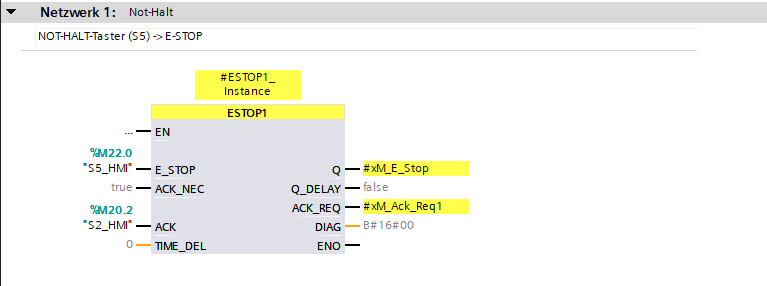
\includegraphics[width=0.9\textwidth]{Bilder/3. Programm/2. Safety/safety_1.png}}
   \caption[Not-Halt FB]{Sicherer Funktionsbaustein für Not-Halt-Funktionalität}
   \label{fig:Bild7.10}
\end{figure}

\begin{figure}[H]
   \centering
   \fbox{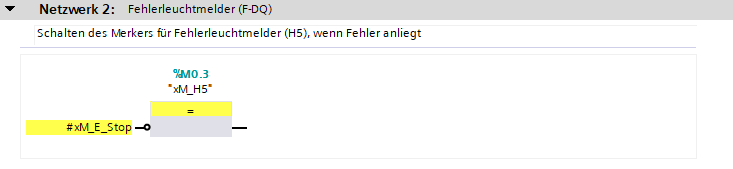
\includegraphics[width=0.9\textwidth]{Bilder/3. Programm/2. Safety/safety_2.png}}
   \caption[Fehlerleuchtmelder]{Netzwerk zur Implementierung des Fehlerleuchtmelders}
   \label{fig:Bild7.11}
\end{figure}

Netzwerk 3 und 4 (\autoref{fig:Bild7.12} und \autoref{fig:Bild7.13}) zeigen die Beschaltung der Schütze für die Schnecke (K3) und das Förderband (K4) sowie deren zugehörigen Leuchtmelder (H3 und H4). Grundsätzlich gilt, dass wenn ein Not-Halt (xM\_E\_Stop) ausgelöst wurde, dass beide Schütze und deren zugehörige Betriebsmittel per \texttt{FALSE}-Signal abgeschaltet werden müssen. Im Falle der Förderschnecke gilt weiterhin, dass diese deaktiviert wird, wenn der Endlagenschalter der Schnecke (B1) oder der Endlagenschalter des Förderbandes (B2) oder beide gleichzeitig ausgelöst sind. \\
Das Förderband kann lediglich zusätzlich zum Not-Halt über die Endlage des Förderbandes (B2) deaktiviert werden. \\
Die Ansteuerung im Normalbetrieb erfolgt über die Merkervariablen \textit{xM\_K3} \bzw \textit{xM\_K4}, die im Standard- Anwenderprogramm gesetzt werden.

\begin{figure}[H]
   \centering
   \fbox{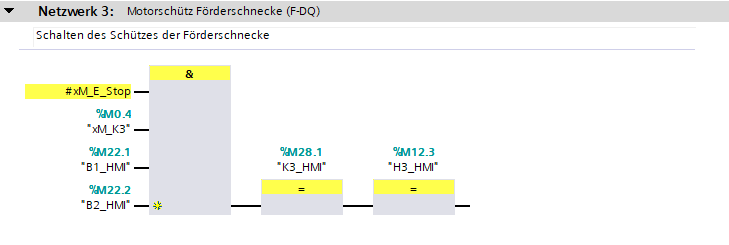
\includegraphics[width=0.9\textwidth]{Bilder/3. Programm/2. Safety/safety_3.png}}
   \caption[Motorschütz Förderschnecke]{Netzwerk zur Ansteuerung des Motorschützes der Förderschnecke}
   \label{fig:Bild7.12}
\end{figure}

\begin{figure}[H]
   \centering
   \fbox{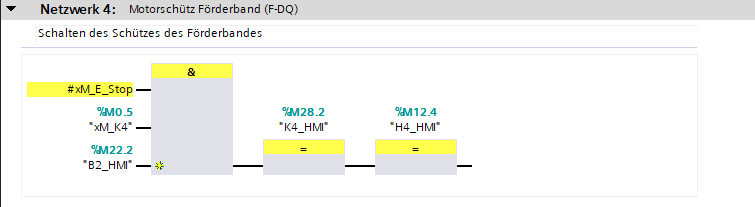
\includegraphics[width=0.9\textwidth]{Bilder/3. Programm/2. Safety/safety_4.png}}
   \caption[Motorschütz Förderband]{Netzwerk zur Ansteuerung des Motorschützes des Förderbandes}
   \label{fig:Bild7.13}
\end{figure}

Die Netzwerke 5 und 6 (siehe \autoref{fig:Bild7.14} und \autoref{fig:Bild7.15}) beinhalten jeweils eine einfache Zuweisung der beiden F-Variablen der Endlagenschalter (B1 und B2) zu Merkervariablen (xM\_B1 und xM\_B2), die im Standard- Anwenderprogramm nun weiterverwendet werden können. Auch die Endlagen sind zweikanalig ausgeführt und jeweils der Öffner-Kontakt ist mit der Variablen verknüpft, weshalb hier noch Negationen hinzugefügt wurden, um das Anwenderprogramm nicht unnötig zu verkomplizieren.

\begin{figure}[H]
   \centering
   \fbox{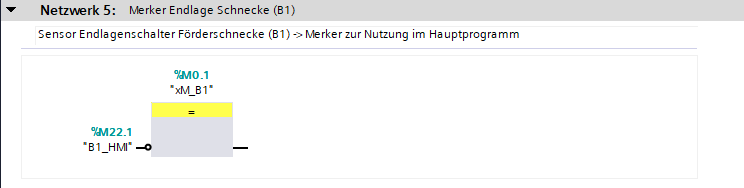
\includegraphics[width=0.9\textwidth]{Bilder/3. Programm/2. Safety/safety_5.png}}
   \caption[Merker Endlage Förderschnecke]{Zuweisung des Sensorsignals der Förderschnecke zu einer Merkervariable}
   \label{fig:Bild7.14}
\end{figure}

\begin{figure}[H]
   \centering
   \fbox{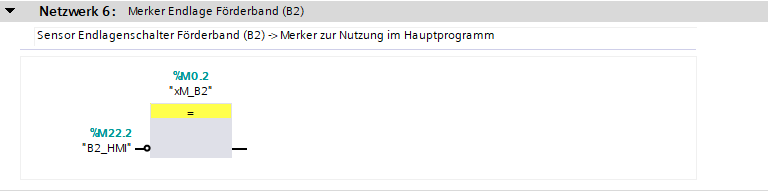
\includegraphics[width=0.9\textwidth]{Bilder/3. Programm/2. Safety/safety_6.png}}
   \caption[Merker Endlage Förderband]{Zuweisung des Sensorsignals des Förderbandes zu einer Merkervariable}
   \label{fig:Bild7.15}
\end{figure}

In den Netzwerken 7 und 8 (\autoref{fig:Bild7.16} und \autoref{fig:Bild7.17}) findet eine Diskrepanzanalyse zwischen jeweils den Schützen und den Rückmeldungen der Schütze statt (K3 und B3 \bzw K4 und B4). Es soll folglich ermittelt werden, ob die Werte der jeweils zusammengehörigen booleschen Variablen voneinander abweichen, um zu ermitteln, ob ein Anlagenfehler vorliegt. Dazu wird der Funktionsbaustein \textbf{EV1oo2DI} verwendet. Der Baustein besitzt für uns fünf relevante Eingänge. Zunächst \textbf{IN1} und \textbf{IN2}, welche die beiden Eingangsvariablen (\zB K3 und B3) entgegennehmen, die auf eine Diskrepanz überwacht werden sollen. Über \textbf{DISCTIME} kann eingestellt werden, nach welcher Zeit eine Diskrepanz zwischen den beiden Eingängen zum Auslösen eines Fehlers vergehen muss. Hier wurden konkret zunächst 500 ms eingesetzt, um zu berücksichtigen, dass die Schütze bei einer realen Anlage eine gewisse Zeit benötigen, um zu Schalten. Wie auch schon beim Not-Halt wird hier der Eingang \textbf{ACK\_NEC} auf \texttt{TRUE} gesetzt, so dass ein Fehler zunächst eine Quittierung erfordert. Am Eingang \textbf{ACK} wird erneut der Quittier-Drucktaster (S2) eingesetzt, um einen Diskrepanzfehler quittieren zu können. \\
Von den Ausgängen des Funktionsbausteins werden lediglich zwei benötigt. Zum Einen für das Quittieren der Ausgang \textbf{ACK\_REQ}, wenn nach einem Diskrepanzfehler dieser quittiert werden kann. Hier wird auch wieder eine Merkervariable eingesetzt (xM\_Ack\_Req2 \bzw xM\_Ack\_Req3), welche in Netzwerk 10 (siehe \autoref{fig:Bild7.19}) mit dem anderen Quittier-Merker verodert werden. Zum Anderen der Ausgang \textbf{DISC\_FLT}, welcher ein \texttt{TRUE}-Signal ausgibt, wenn eine eine Diskrepanz zwischen den beiden Eingängen \textit{IN1} und \textit{IN2} vorliegt und ein \texttt{FALSE}-Signal, wenn die Eingänge identische Signalwerte besitzen.

\begin{figure}[H]
   \centering
   \fbox{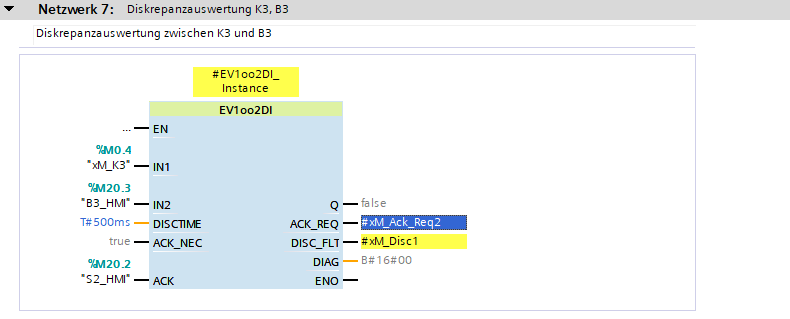
\includegraphics[width=0.9\textwidth]{Bilder/3. Programm/2. Safety/safety_7.png}}
   \caption[Diskrepanzauswertung Schütz Förderschnecke]{Funktionsbaustein zur Diskrepanzauswertung des Schütz-Schaltzustandes der Förderschnecke mit dem Rückmeldesignal des Schützes}
   \label{fig:Bild7.16}
\end{figure}

\begin{figure}[H]
   \centering
   \fbox{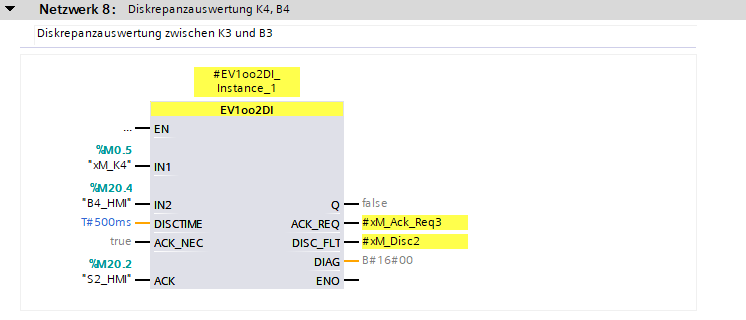
\includegraphics[width=0.9\textwidth]{Bilder/3. Programm/2. Safety/safety_8.png}}
   \caption[Diskrepanzauswertung Schütz Förderband]{Funktionsbaustein zur Diskrepanzauswertung des Schütz-Schaltzustandes des Förderbandes mit dem Rückmeldesignal des Schützes}
   \label{fig:Bild7.17}
\end{figure}

In Netzwerk 9 (siehe \autoref{fig:Bild7.18}) werden die Merkervariablen (xM\_Disc1 und xM\_Disc2) der Ausgänge der Diskrepanzanalyse (DISC\_FLT) miteinander verodert. Liegt folglich mindestens eine Abweichung vor zwischen Schütz und Rückmeldung, so wird die Merkervariable für den Not-Halt (xM\_E\_Stop) gesetzt.

\begin{figure}[H]
   \centering
   \fbox{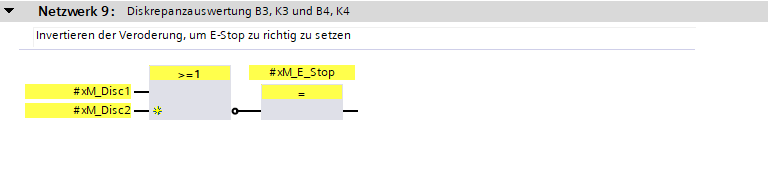
\includegraphics[width=0.9\textwidth]{Bilder/3. Programm/2. Safety/safety_9.png}}
   \caption[Globale Diskrepanzauswertung]{Vereinigung der Diskrepanzauswertungen zu einer Globalen Diskrepanzauswertung der Eingangssignale}
   \label{fig:Bild7.18}
\end{figure}

Netzwerk 10 (\autoref{fig:Bild7.19}) zeigt wie bereits erwähnt die Veroderung der Quittier-Aufforderungen (Ack\_Req). Ist mindestens ein Signal auf \texttt{TRUE}, wird der Nutzer aufgefordert den jeweils aufgetretenen Fehler zu quittieren.

\begin{figure}[H]
   \centering
   \fbox{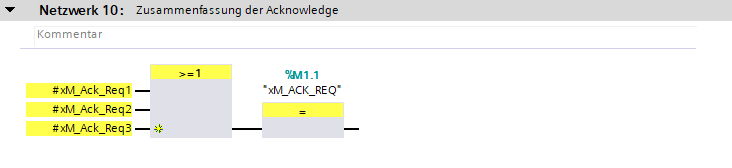
\includegraphics[width=0.9\textwidth]{Bilder/3. Programm/2. Safety/safety_10.png}}
   \caption[Vereinigung Quittieraufforderungen]{Vereinigung der Signale zur Quittieraufforderung}
   \label{fig:Bild7.19}
\end{figure}

Das letzte Netzwerk des Sicherheitsprogramms (siehe \autoref{fig:Bild7.20}) zeigt den Funktionsbaustein zum globalen Quittieren von Fehlern. Über diesen können alle F-Peripherie und F-Ablaufgruppen wieder eingegliedert werden nach \zB einem Kanalfehler mit anschließender Passivierung. Der Baustein besitzt lediglich einen Eingang (\textbf{ACK\_GLOB}). Auch an diesem wird der Quittier-Taster (S2) eingesetzt.

\begin{figure}[H]
   \centering
   \fbox{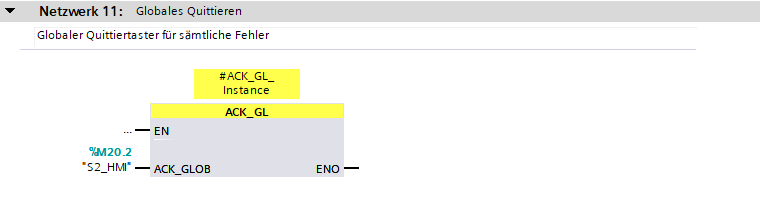
\includegraphics[width=0.9\textwidth]{Bilder/3. Programm/2. Safety/safety_11.png}}
   \caption[FB zum globalen Quittieren]{Sicherer Funktionsbaustein zur Umsetzung einer globalen Quittierfunktionalität}
   \label{fig:Bild7.20}
\end{figure}

\clearpage

\subsection{Visualisierung}

Da zum Zeitpunkt der Dokumentationserstellung keine reale Anlage zur Verfügung stand, wurde mit der SIMATIC HMI eine Visualisierung angefertigt (\autoref{fig:Bild7.21}). Die Visualisierung spiegelt den realen Aufbau wieder. Zur Überprüfung der Schütze (K3, K4), wurden zwei weitere Leuchtmelder eingefügt. Diese sind in der realen Anlage nicht vorhanden. Im Gegensatz zur realen Anlage können durch die Visualisierung nicht alle Sachverhalte korrekt dargestellt werden. Somit sind die Öffner-Taster mit dem Kommentar \glqq Toggle\grqq\:versehen, da in der Simulation keine öffnenden Taster eingefügt werden können. Bei der Bedienung ist darauf zu achten, dass ein Klicken das jeweilige Bit nur invertiert! Die Endlagentaster des Förderbands und der Förderschnecke sind durch B1 und B2 dargestellt und ebenfalls mit einem Kommentar versehen worden. 

\begin{figure}[H]
   \centering
   \fbox{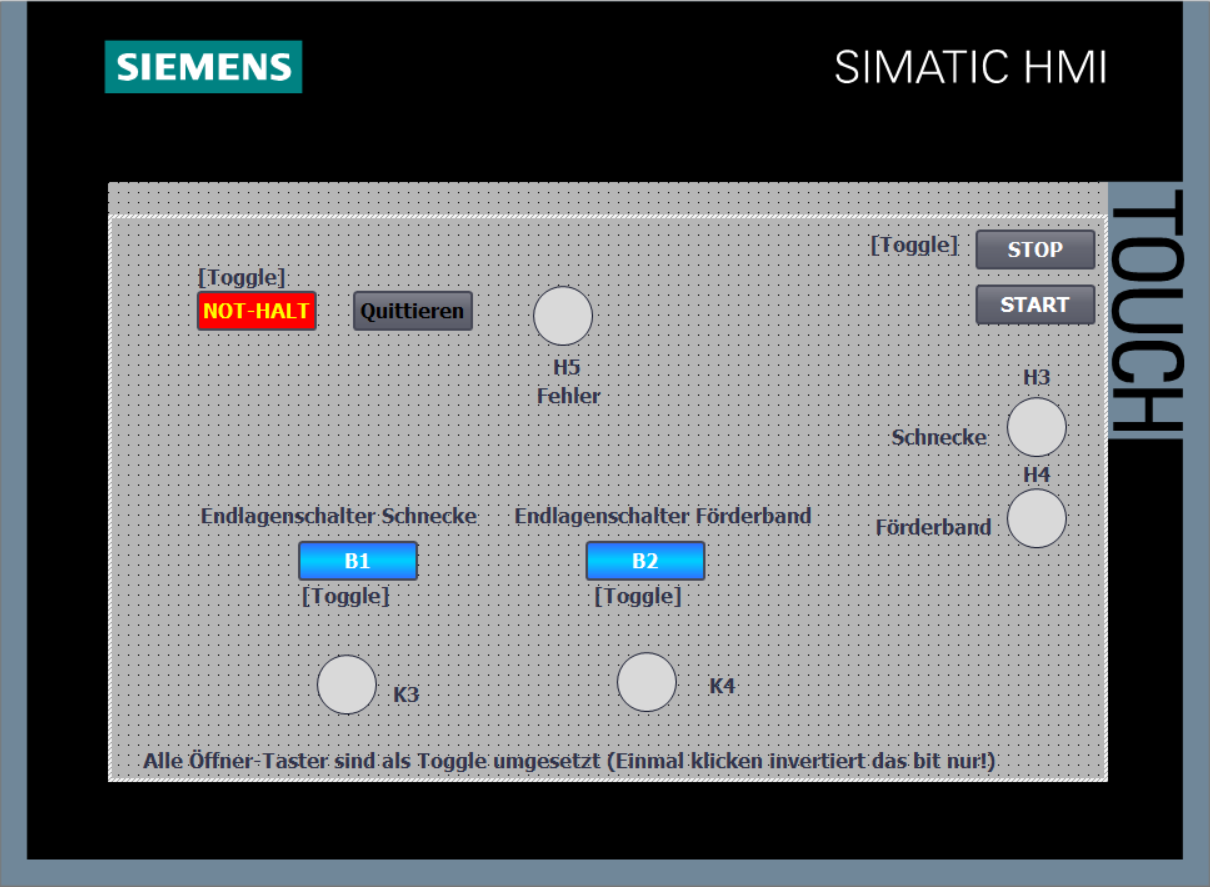
\includegraphics[width=0.8\textwidth]{Bilder/3. Programm/3. Visualisierung/Visualisierung_HMI.png}}
   \caption[Visualisierung mit SIMATIC HMI]{Visualisierung mit SIMATIC HMI unter Nutzung der Software WinCC}
   \label{fig:Bild7.21}
\end{figure}
